\section{Thuật toán Shift Or}

\subsection{Đặc điểm chính}

Thuật toán Shift-Or (còn được gọi là Shift-And) là một thuật toán tìm kiếm chuỗi dựa trên phép toán bit (bitwise operations), được sử dụng để xác định sự xuất hiện của xâu mẫu trong văn bản một cách hiệu quả. Thuật toán này đặc biệt phù hợp khi độ dài của xâu mẫu không quá lớn và có thể được biểu diễn bằng các bit trong một từ máy.

Thuật toán hoạt động bằng cách biểu diễn trạng thái khớp của các ký tự trong mẫu dưới dạng các phép dịch bit và phép toán logic AND/OR. Nhờ đó, quá trình so khớp ký tự được thực hiện song song ở mức bit, giúp tăng tốc độ xử lý so với các phương pháp so sánh tuần tự truyền thống.

Thuật toán Shift-Or có các đặc điểm sau:

\begin{itemize}
    \item Sử dụng các kỹ thuật thao tác bit (bitwise techniques) để thực hiện so khớp.
    \item Hiệu quả khi độ dài của xâu mẫu không vượt quá kích thước từ nhớ (word size) của máy tính.
    \item Giai đoạn tiền xử lý có độ phức tạp $O(m + \sigma)$ về cả thời gian và không gian, trong đó $m$ là độ dài xâu mẫu và $\sigma$ là kích thước bảng chữ cái.
    \item Giai đoạn tìm kiếm có độ phức tạp $O(n)$, không phụ thuộc vào kích thước bảng chữ cái hay độ dài xâu mẫu.
    \item Dễ dàng mở rộng để áp dụng cho bài toán tìm kiếm xâu xấp xỉ (approximate string matching).
\end{itemize}

\subsection{Mô tả thuật toán}

Thuật toán Shift Or sử dụng thao tác bit. Gọi $R$ là mảng bit có kích thước $m$. Vector $R_j$ là giá trị của mảng $R$ sau khi ký tự $y[j]$ đã được xử lý. Vector này chứa thông tin về tất cả các tiền tố của $x$ mà kết thúc tại vị trí $j$ trong xâu, với $0 <i\leq m - 1$

Ta có công thức sau:

\[
R_j[i] =
\begin{cases}
0 & \text{if } x[0..i] = y[j-i..j] \\
1 & \text{otherwise}
\end{cases}
\]

Vector $R_{j+1}$ có thể được tính từ $R_j$ như sau.
Với mỗi vị trí mà $R_j[i] = 0$, ta có:

\[
R_{j+1}[i+1] =
\begin{cases}
0 & \text{if } x[i+1] = y[j+1] \\
1 & \text{otherwise}
\end{cases}
\]

và

\[
R_{j+1}[0] =
\begin{cases}
0 & \text{if } x[0] = y[j+1] \\
1 & \text{otherwise}
\end{cases}
\]

Nếu $R_{j+1}[m-1]=0$ thì một chuỗi so khớp sẽ được ghi nhận.

\begin{figure}[H]
    \centering
    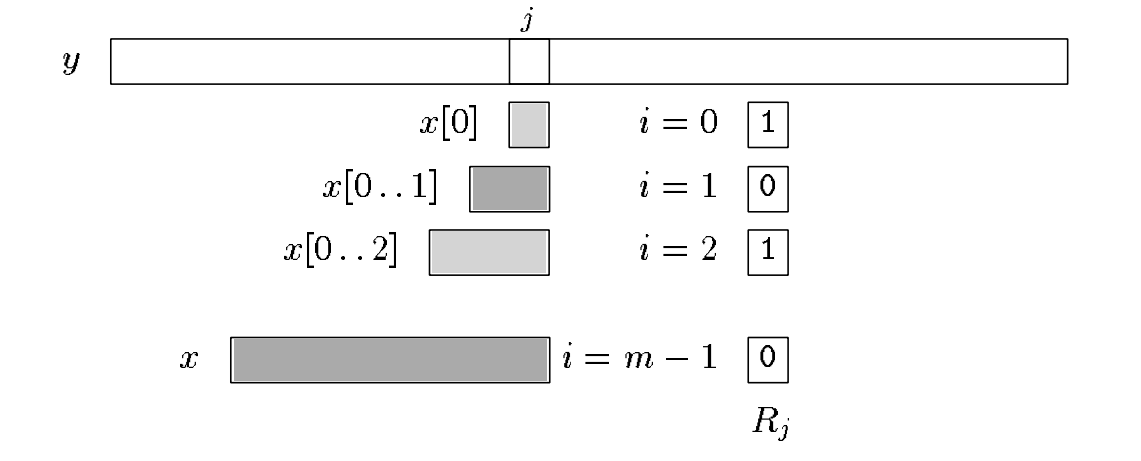
\includegraphics[width=12cm]{Images/shift_or_1.png}
    \caption{Minh họa cập nhật vector $R_j$ trong thuật toán Shift-Or}
    \label{fig:shift-or-update}
\end{figure}

Chuyển từ $R_j$ sang $R_{j+1}$ có thể tính toán rất nhanh dựa theo: Với mỗi $c \in \Sigma$, gọi $S_c$ là một vector bit có kích thước $m$ thỏa mãn:

với $0 \leq i \leq m - 1$, $S_c[i] =0$ khi và chỉ khi $x[i] = c$.

Mảng $S_c$ chỉ ra các vị trí của của ký tự $c$ trong xâu mẫu $x$. Mỗi $S_c$ có thể được tiền xử lý trước khi tìm kiếm. Và quá trình tính toán của $R_{j+1}$ được giảm xuống còn 2 thao tác, $\texttt{shift}$ và $\texttt{or}$:

\[
R_{j+1} = \text{SHIFT}(R_j) \text{ OR } S_{y[j+1]}
\]

Giả sử độ dài mẫu không vượt quá kích thước từ nhớ (machine word) của máy, giai đoạn tiền xử lý yêu cầu độ phức tạp thời gian và không gian là \(O(m + \sigma)\).

Giai đoạn tìm kiếm có độ phức tạp thời gian \(O(n)\), không phụ thuộc vào kích thước bảng chữ cái và độ dài mẫu.

\subsection{Cài đặt thuật toán bằng C++}
\begin{verbatim}
#include <iostream>
#include <vector>
#include <string>

using namespace std;

const int ASIZE = 256;

vector<int> shiftOr(const string& pattern, const string& text) {
    int m = pattern.length();
    int n = text.length();

    if (m > 31) {
        throw runtime_error("Pattern length must not exceed word size");
    }

    vector<unsigned int> mask(ASIZE, ~0);

    unsigned int state = ~0;
    unsigned int lim = 0;

    /*
     * Preprocessing phase
     */
    unsigned int bit = 1;

    for (int i = 0; i < m; ++i) {
        mask[(unsigned char)pattern[i]] &= ~bit;
        lim |= bit;
        bit <<= 1;
    }

    lim = ~(lim >> 1);

    /*
     * Searching phase
     */
    vector<int> occurrences;

    for (int j = 0; j < n; ++j) {
        state = (state << 1) | mask[(unsigned char)text[j]];

        if (state < lim) {
            occurrences.push_back(j - m + 1);
        }
    }

    return occurrences;
}

int main() {
    string text = "ababcabcabababd";
    string pattern = "ababd";

    vector<int> result = shiftOr(pattern, text);

    for (int pos : result) {
        cout << "Pattern found at position: " << pos << endl;
    }

    return 0;
}
\end{verbatim}

\subsection{Đánh giá độ phức tạp của thuật toán}
Giả sử độ dài mẫu không lớn hơn kích thước của từ nhớ máy tính.
\begin{itemize}
    \item Độ phức tạp pha tiền xử lý là $O(m + \sigma)$.
    \item Độ phức tạp của pha tìm kiếm là $O(n)$.
\end{itemize}

\subsection{Kiểm nghiệm thuật toán}
Tính các vector $S_c$:

\begin{figure}[H]
    \centering
    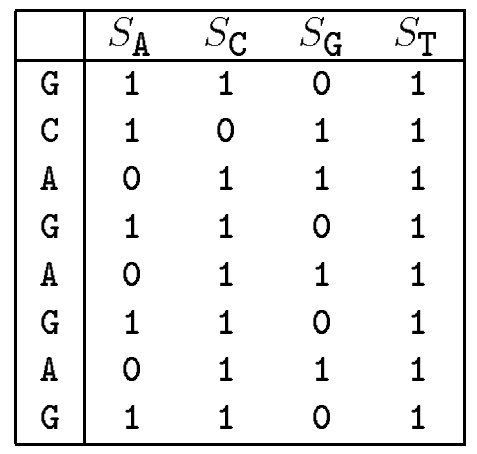
\includegraphics[width=10cm]{Images/shift_or_2.png}
    \caption{Các vector $S_c$ trong thuật toán Shift-Or}
    \label{fig:shift-or-sc-vectors}
\end{figure}

Tính các vector $R_j$:

\begin{figure}[H]
    \centering
    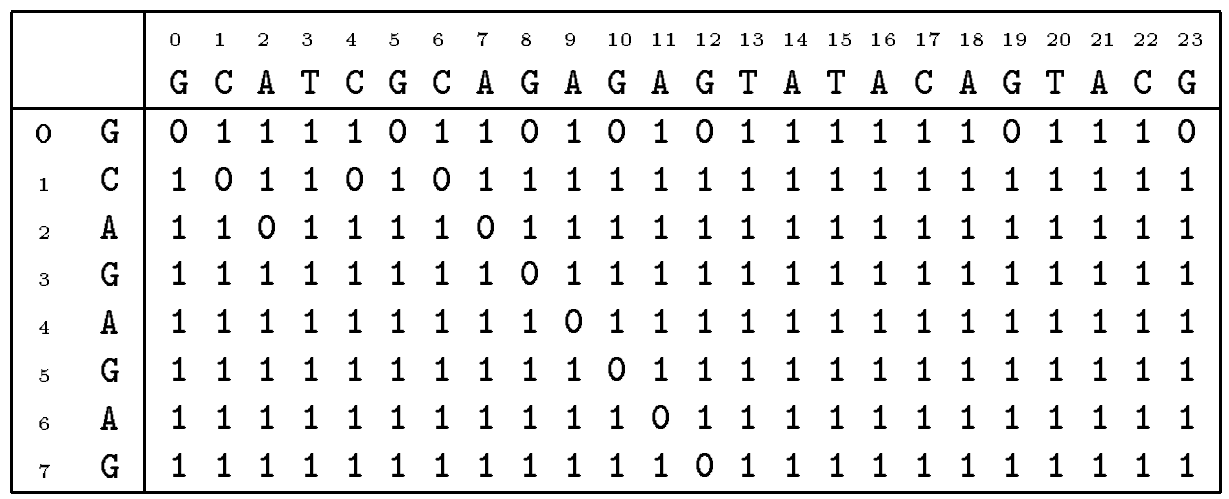
\includegraphics[width=10cm]{Images/shift_or_3.png}
    \caption{Các vector $R_j$ trong thuật toán Shift-Or}
    \label{fig:shift-or-rj-vectors}
\end{figure}

Với $R_12[7] = 0$ tức là $x$ được tìm thấy tại vị trí $12 - 8 + 1 = 5$.